\section{Introduction}
Officially completed in September 2017, the 12 GeV upgrade project of Jefferson Lab consists not only in the increase 
of energy of its Continuous Electron Beam Accelerator Facility (CEBAF) from 6 to 12 GeV, but also in the construction 
or upgrades of its experimental Halls. Hall B, which is the focus of this status report, updated its existing CLAS 
spectrometer with new magnets and detectors to capture the more forward-focused reaction products at an increased 
luminosity. This new spectrometer called CLAS12 became fully operational in the Fall of 2017 and started its 
engineering run in December. CLAS12 is now taking data as part of the run group A, which focus is on the study of the 
3-dimensional structure of the nucleon using Deeply Virtual Compton Scattering (DVCS) on the proton.

As early as 2006, the Irfu group started studying the feasibility of a Central Tracker for CLAS12 based on the use of 
cylindrical layers of Micromegas detectors in addition to the Silicon Vertex Tracker being designed at JLab. In 2010, a 
full proposal was submitted to the CSTS as well as to the JLab management and it was decided that the baseline design 
for the central tracker would consist in 3 double-layers of Silicon Vertex Tracker (SVT) displayed in polyhedral 
arrangement, followed by six layers of cylindrical Barrel Micromegas Tracker (BMT), which benefits from the 
specificities of both technologies as foreseen in early simulations. This central tracker would also be completed with 
a Forward Micromegas Tracker (FMT) in order to tag forward tracks and improve the vertex and angle resolutions in the 
fringe field of the solenoid magnet. This forward part consists in 6 identical Micromegas disks. This report focuses on 
the status of the CLAS12 Micromegas tracker project, including both the BMT and FMT systems, recently fully installed 
and commissioned. The Barrel and the Forward Micromegas Tracker forms together the Micromegas Vertex Tracker.

\section{System description}

\subsection{General}


The Barrel Micromegas Tracker consists of six layers of cylindrical detectors, three with strips along the beam axis (Z 
strips) and three with circular strips (C strips) perpendicular to the beam axis. Each layer is made of three curved 
120$^o$ detectors. A total of 18 curved detectors are assembled on a carbon, stainless-steel and peek structure to 
complete the Barrel. The Micromegas detectors are ``resistive'', a coating of resistive material is deposited on the 
top of the readout strip thus allowing to operate the detectors without spark at high rate. In this configuration the 
mesh is grounded and the high voltage for amplification is positive on the resistive strips.

\begin{figure}[htb]
 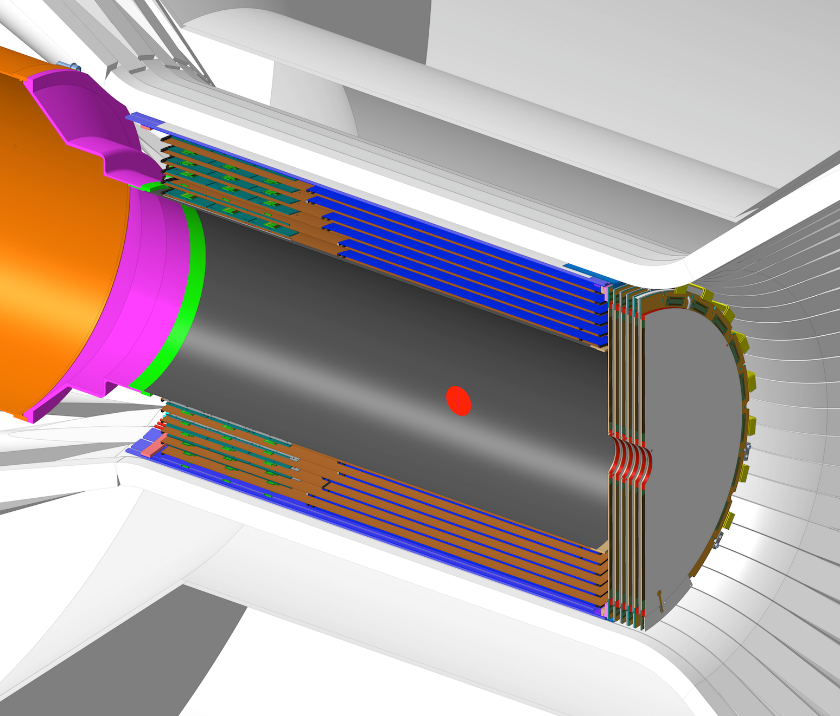
\includegraphics[width=1.0\columnwidth,keepaspectratio]{images/fig1}
 \caption{Cut view showing the 6 different layers of BMT and 6 identical FMT disks. It is shown inserted close to the 
central Time-of-Flight, itself in the 5T solenoid magnet.}
 \label{fig:mm-fig1}
\end{figure}

The Forward Micromegas Tracker consists of six flat Micromegas disks stacked together. The disks are all identical and 
assembled with a 60$^o$ rotation with respect to one another giving 3 angles of strips (0$^o$, 60$^o$ and 120$^o$). The 
resulting Micromegas Forward tracker is attached to the Barrel end flange. Figure \ref{fig:mm-fig1} displays a cut view 
showing all types of detectors for both BMT and FMT.

\subsection{Mechanical strucutre}
In order to hold the Micromegas Vertex Tracker in the magnet, a stainless-steel tube with the Barrel and Forward at 
its downstream end is attached to the flange of the SVT tube structure, as shown on Figure \ref{fig:mm-fig2}. This tube 
also holds the 6 crates containing the 48 readout Front End Unit (FEU) boards for the Micromegas detectors. The 
connection between detectors and readout FEU is done using flex cables. Each FEU is connected to Back End Unit with a 
fiber optic. The patch panels for the gas and the high voltage cables are located on the 6 crates.

\begin{figure}[htb]
 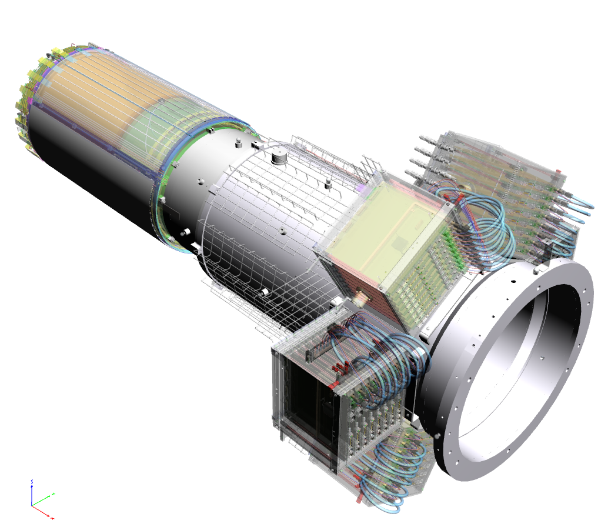
\includegraphics[width=1.0\columnwidth,keepaspectratio]{images/fig2}
 \caption{Support tube with electronics rack and MVT detectors.}
 \label{fig:mm-fig2}
\end{figure}

The mechanics of the Barrel structure is made of thin (1 mm) carbon cylinder with a glued Peek flange downstream, and a 
glued stainless-steel flange upstream, as shown on Figure \ref{fig:mm-fig3}. The goal was to minimize the material 
budget in the detection region. The stainless steel used for the tube and flanges is made of 904L (non-magnetic steel). 
Detectors (barrels and forwards) and the tube are equipped with fixation for laser tracker targets, thus allowing the 
survey team to locate the strips position from the rear of the tube to a precision of around 0.3mm. The final alignment 
is done using cosmic rays or low rate beam data. 

\begin{figure}[htb]
 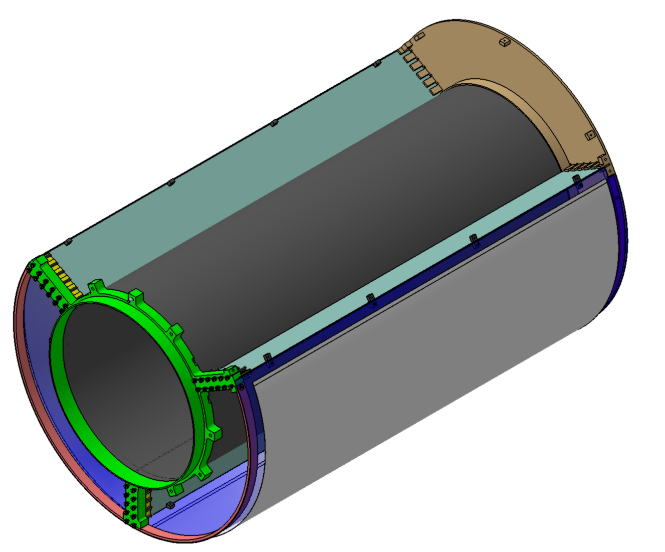
\includegraphics[width=1.0\columnwidth,keepaspectratio]{images/fig3}
 \caption{BMT mechanical structure, one sector open to house 6 curved detectors.}
 \label{fig:mm-fig3}
\end{figure}


\subsection{Barrel Micromegas Tracker (BMT)}

The Barrel detectors are made of a thin PCB (0.2 mm) transformed in Micromegas with the bulk process. MEC8 connectors 
are welded on one side and on each longitudinal side of the PCB a square carbon tube is glued. The PCB is curved on a 
homemade mandrel tool with the wanted radius and four arches, two made out of carbon and two of aluminum, are glued to 
obtain a curved Micromegas bulk. The carbon and aluminum structure thickness, 3 mm, defines the drift gap of the 
detectors. A Kapton foil (0.25 mm) with metallic coating is then glued on top of the carbon-aluminum structure to seal 
the detectors and to do the drift of the detector. A curved plastic mechanics, made by 3 D printing, is assemble above 
the connectors to provide rigidity for the connection of signal cables. A metallic box with the high voltage contact 
and “protection circuit” is fixed on the side of the PCB.  Gas is introduced by the downstream side and flush out 
downstream through the hollow carbon-aluminum mechanical structure. The leak rate of each detector is measured bellow 
2.10-3 l/h.  On both ends of each carbon tube of the detectors are inserted and glued pin in order to fasten and 
localize the detectors to the barrel structure. Figure \ref{fig:mm-fig5} shows a view of curved BMT detectors.

\begin{figure}[htb]
 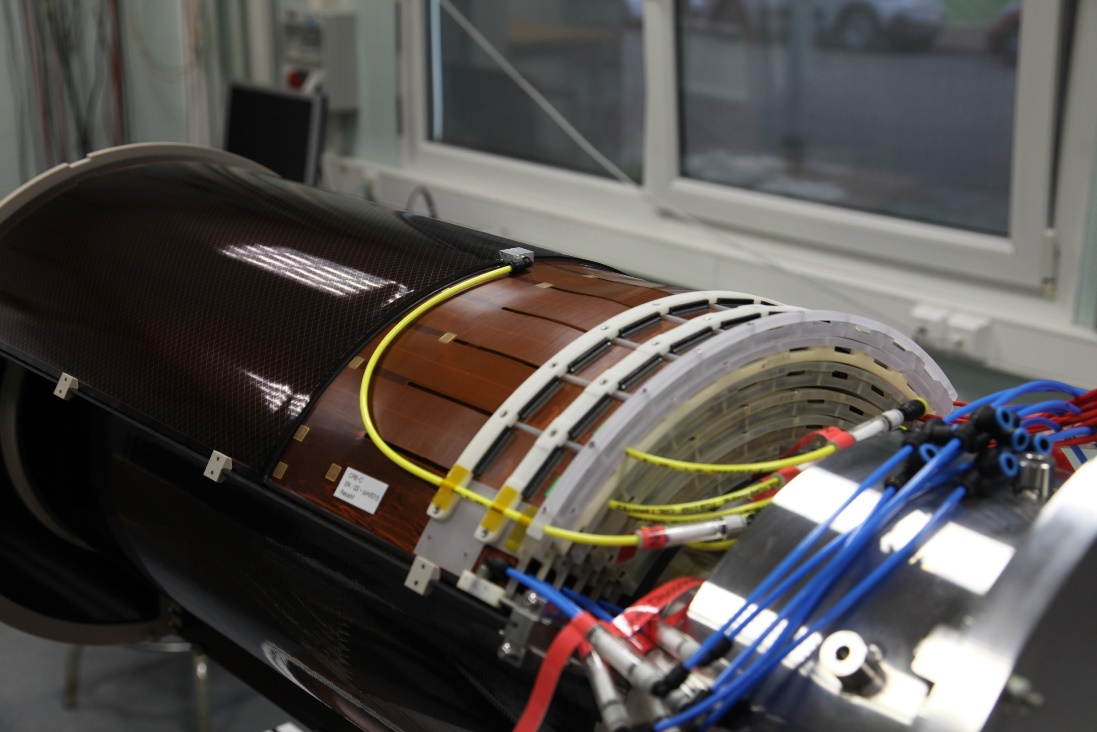
\includegraphics[width=1.0\columnwidth,keepaspectratio]{images/fig5}
 \caption{Full stack of 6 BMT layers in its mechanics.}
 \label{fig:mm-fig5}
\end{figure}

As pointed out before, the BMT is located inside the 5T solenoid used as a Moller shield. This situation had a strong 
consequence for the design and use of the BMT detectors: indeed, the (detector) electric and (solenoid) magnetic fields 
being essentially orthogonal, the primary electrons in the drift region of the Micromegas detectors are subject to a 
Lorentz angle, that make them drift transversally, therefore spreading the charge over a large area and directly 
impacting the position resolution and even the efficiency in extreme cases. Early studies by our group showed that 
strong Lorentz angles could be partly compensated by using a large drift high voltage \cite{KONCZYKOWSKI2010274}. The 
effect is worst in the case of Z-type detectors with strips parallel to the B-field direction: in that particular case, 
we concluded that we needed to reach drift HV in the range 1500-2000V to minimize the effect.

\subsection{Forward Micromegas Tracker (FMT)}

The Forward Micromegas Tracker, shown in Figure 6 (middle), consists of six identical Micromegas resistive detectors in 
the forward region from 30 cm to 36 cm of the target center. Each Micromegas detector, shown in Figure 6 (left and 
right), is a 450 mm diameter disk with an active area of 1024 readout strips (525 $\mu$m pitch) in one projection. 
Signals are read out via 16 connectors. The next disk is rotated of 60 degrees relative to the previous one with a 10.5 
mm space between their two active areas. 

\begin{figure}[htb]
 
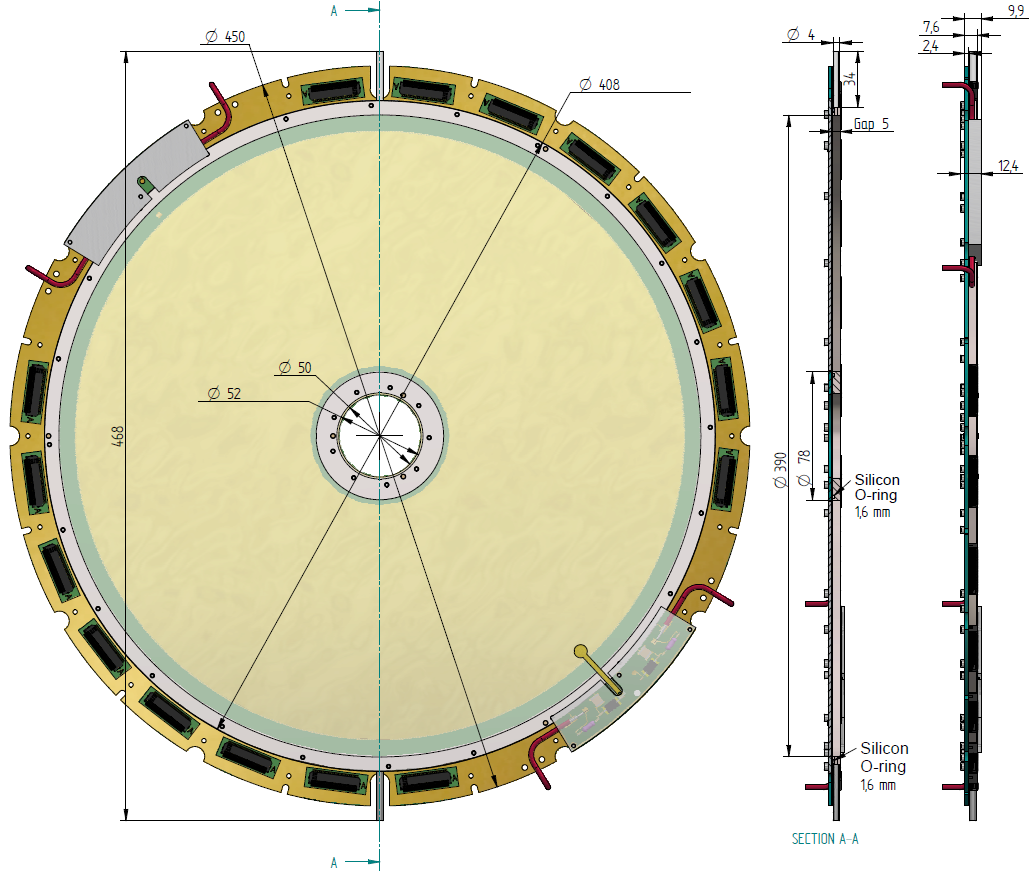
\includegraphics[width=0.66\columnwidth,keepaspectratio]{images/fig6_1}~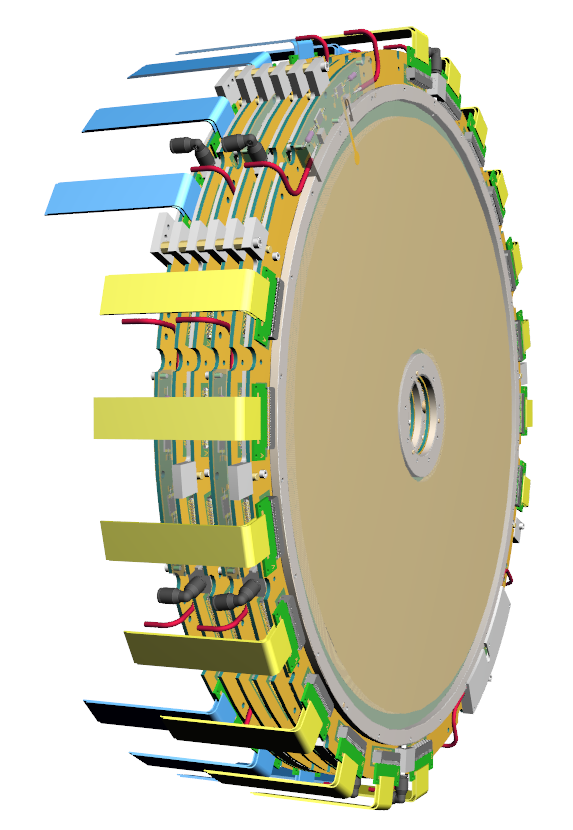
\includegraphics[width=0.33\columnwidth,
keepaspectratio]{images/fig6_2}
 \caption{CAD views of a FMT disks.}
 \label{fig:mm-fig5}
\end{figure}

By convention, the Micromegas detector are numbered from 1 to 6, (number 1 close to the target). The active area is 
divided in two parts, the inner part (IN),  diameter  $86 < d < 66$ mm, and the outer part (OUT), $168 < d < 380$ mm. 
In operation, a Micromegas detector has to be polarized by three high voltages (HV), the two active areas corresponding 
to the anode and the drift plane (cathode) 5 mm above the anode. The inner region can be disabled in case of pile-up 
(very high flux).


\subsection{Gas system}

The Micromegas are continuously flushed with gas in order to keep a good purity and overcome the normal outgassing of 
the detectors. The gas used for the barrel detector is a flammable mixture, argon with 10\% of isobutane. For the 
forward detector, it is argon with 10\% of CF4 and 10\% of isobutane. The flow rate is 2 l/h (liter per hour) for a set 
of three detectors in serial. For the barrel 6 lines, one for each layer, and 2 for the forward, of pipes allows the 
flushing, thus a total of $\sim$ 20 l/h is used.  The gas is rejected outside Hall B. An MVT gas control panel located 
in the closet with the MVT back-end electronics allows to operate the gas rack in manual (with fixed values for the 
flow and pressure) or in automatic mode controlled by a PLC for each sub system (Barrel and Forward) Due to the small 
thickness of curved detectors, the flow rate and pressure must be low and controlled to avoid any deformation on the 
detectors. The nominal pressure is 2 mbar above atmosphere and the flow rate is 2 l/h.